\section{Zustandsraumdarstellung \tiny{$Revision: 1352 $}}
\scriptsize
\label{sec:ZRD}

\subsection{Basics}
Darstellung einer Differentialgleichung $n$. Ordnung durch ein
Differentialgleichungssystem von $n$ Gleichungen 1. Ordnung.


\begin{figure}[!h]
	\normalsize
	\begin{minipage}{.45\linewidth}
		\centering
		\normalsize
		\subfloat{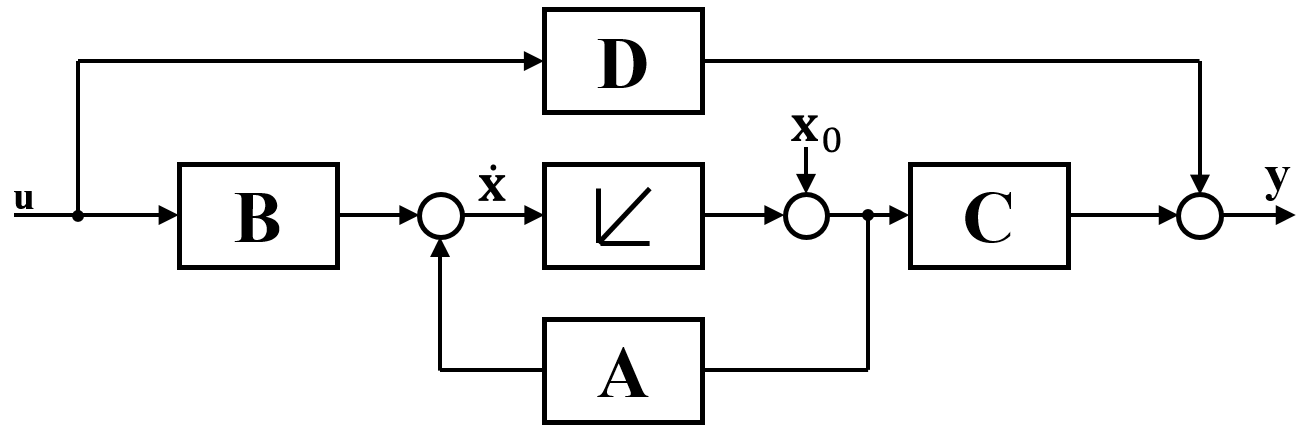
\includegraphics[width=\linewidth]{./bilder/zrd.png}}
	\end{minipage}%
	\hfill
	\begin{minipage}{.45\linewidth}
		$\dot{\underline{x}}(t) = {\boldsymbol A} \underline{x}(t) + {\boldsymbol B}
		\underline{u}(t)$\newline
		$\underline{y}(t) = {\boldsymbol C} \underline{x}(t) + {\boldsymbol D}
		\underline{u}(t)$\\ \\
		Pole des Systems: Eigenwerte von $\boldsymbol{A}$\\
		$\det\left(\lambda \boldsymbol{I}- \boldsymbol{A}\right) =0$
	\end{minipage}
	\caption{Zustandsraumdarstellung}
	\label{fig:ZRD}
\end{figure}



\begin{tabularx}{\linewidth}{lllX}\hline
	\textbf{Matrix}			&\textbf{Dimension}		&\textbf{Einfluss}					&\textbf{Weiteres}\\\hline
	${\boldsymbol A}$		&$n \times n$			&Beschreibt Dynamik des Systems 	& Spalten entsprechen Ausgängen der Intergratoren\newline Zeilen deren Eingänge\\\hline
	${\boldsymbol B}$		&$n \times M$			&Einfluss der Eingangsvariablen auf Zustandsvariablen 	& Steuer- oder Eingangsmatrix\\\hline
	${\boldsymbol C}$		&$P \times n$			&Einfluss der Zustandsvariablen auf Ausgangsgrössen		& Beobachtungs- oder Ausgangsmatrix\\\hline
	${\boldsymbol D}$		&$P \times M$			&Direkter Einfluss der Eingangsvariablen auf Ausgangsvariablen & Übergangs- oder Durchgangsmatrix\\\hline
\end{tabularx}\\
Dabei gilt:\hspace{5mm}
$n$ = Anzahl Zustandsvariablen; \hspace{5 mm}
$M$ = Anzahl Eingangsvariablen; \hspace{5 mm}
$P$ = Anzahl Ausgangsvariablen
\subsubsection{Stabilität}
Ein LTI-System ist asymptotisch stabil wenn der Realanteil aller Eigenwerte von A kleiner als Null ist. Die Impulsantwort klingt dann gegen Null ab.
\subsubsection{MIMO-Systeme}
\begin{itemize}
	\item Bei einem MIMO-System ist $\boldsymbol{G}\left(s\right)$ eine $P\times M$-Matrix
	\begin{itemize}
		\item Dabei beschreibt jede der Übertragungsfunktionen den Einfluss eines Eingangs auf den  Ausgang
		\item Somit gilt: \begin{equation*}
		\boldsymbol{G}\left( s \right) = \begin{bmatrix}
		\text{Einfluss Eingang 1 auf Ausgang 1}		&	\text{Einfluss Eingang 2 auf Ausgang 1}&	\cdots& \text{Einfluss Eingang M auf Ausgang 1}\\
		\text{Einfluss Eingang 1 auf Ausgang 2}		&	\text{Einfluss Eingang 2 auf Ausgang 2}& \cdots& \text{Einfluss Eingang M auf Ausgang 2}\\
		\vdots										&	\vdots									&\cdots&	\vdots								\\
		\text{Einfluss Eingang 1 auf Ausgang P}		&	\text{Einfluss Eingang 2 auf Ausgang P}& \cdots &\text{Einfluss Eingang M auf Ausgang P}\\
		\end{bmatrix}
		\end{equation*}
	\end{itemize}
\end{itemize}

\subsection{ZRD zu Übertragungsfunktion (im Bildbereich) }

\begin{equation}
\label{eq:ss2tf}
	\boldsymbol{G}\left( s \right) = \frac{\boldsymbol{Y}\left( s \right)}{\boldsymbol{U}\left( s\right)} = \boldsymbol{C}\left( s\boldsymbol{I}-\boldsymbol{A}\right)^{-1}\boldsymbol{B}+\boldsymbol{D} = \frac{b_{m} s^{m} + b_{m-1} s^{m-1} +\cdots+b_{1} s + b_{0}}{s^{n} + a_{n-1} s^{n-1} + \cdots + a_{1} s + a_{0}}
\end{equation}
\begin{itemize}
	\item Dabei ist $\boldsymbol{I}$ die Einheitsmatrix mit der Dimension von $\boldsymbol{A}$
	\item  Wenn $\boldsymbol{D} \neq 0$, dann ist $b_m \neq 0$ und die Sprungantwort des Systems hat eine Sprungkomponente im Ausgang.
	\item Vorteilhaft in TR: Aus multiplizieren mit Variablen, nicht mit eingesetzten Werten um frühzeitiges Kürzen zu verhindern.
\end{itemize}

\subsection{Übertragungsfunktion zu ZRD}
\begin{itemize}
	\item Matlab: \textit{ss2tf}
	\item Es sind verschiedene Umformungen möglich, sie können die Steuerbarkeit ()\ref{subsubsec:Steuerbarkeit}) oder die Beobachtbarkeit (\ref{subsubsec:Beobachtbarkeit}) garantieren. Für beide oft verwendeten Umformungen muss $G\left( s\right)$ in folgende Form gebracht werden:
\end{itemize}
\begin{equation*}
	G \left( s\right) = \frac{b_{n-1}\cdot s^{n-1}+\ldots+b_1\cdot s+b_0}{s^n+a_{n-1}\cdot s^{n-1}+\ldots+a_1\cdot s+a_0}+d
\end{equation*}
\subsubsection{Steuerbare kanonische Normalform}
Mit dieser Methode umgeformte Systeme sind immer steuerbar
\begin{eqnarray} \nonumber
\boldsymbol{A}_c = 
	\begin{bmatrix}
		0 		& 1 		& 0 		&\cdots & 0\\
		0 		& 0 		& 1 		&\cdots & 0\\
		\vdots	& \ddots	& \ddots	&\ddots	& \vdots\\
		0		&\cdots		&0			&\cdots &1\\
		-a_0	&-a_1		&-a_2		&\cdots	&-a_{n-1}
	\end{bmatrix} &
\boldsymbol{B}_c = 
	\begin{bmatrix}
		0\\
		0\\
		\vdots\\
		0\\
		1
	\end{bmatrix} &
\boldsymbol{C}_c = 
	\begin{bmatrix}
		b_0	& b_1 & b_2 &\cdots &b_{n-1}	
	\end{bmatrix} \hspace{5mm}
	D_c = d
\end{eqnarray}

\subsubsection{Beobachtbare kanonische Normalform}
Mit dieser Methode umgeformte Systeme sind immer beobachtbar
\begin{eqnarray} \nonumber
\boldsymbol{A}_c = 
	\begin{bmatrix}
		0 		& 0 		& \cdots  	&0 		& -a_0\\
		1 		& 0 		& \cdots 	&0 		& -a_1\\
		0		&1			&\cdots 	&0 		& -a_2\\
		\vdots	& \ddots	& \ddots	&\vdots	& \vdots\\
		0		&0			&\cdots		&1		&-a_{n-1}
	\end{bmatrix} &
\boldsymbol{B}_o = 
		\begin{bmatrix}
		b_0\\
		b_1\\
		\vdots\\
		b_{n-2}\\
		b_{n-1}
	\end{bmatrix} &
\boldsymbol{C}_o = 
	\begin{bmatrix}
		0	& 0 & \cdots & 0 &1
	\end{bmatrix} \hspace{5mm}
D_o = d
\end{eqnarray}

\subsubsection{Ähnlichkeitstransformation}
\begin{itemize}
	\item Jedes System ist auf verschiedene Möglichkeiten darstellbar (z.B. sowohl in Beobachtbarer sowie auch in Steuerbarer kanonischer Normalform)
	\item Die Darstellung ist abhängig von der Wahl (und der Reihenfolge) der Zustandsvariablen
	\item Mit einer regulärer ($\Rrightarrow$ invertierbaren) Matrix $\boldsymbol{T}$ kann Darstellung beliebig transformiert werden
	\item[ ] $	\boldsymbol{\tilde{A}} = \boldsymbol{TAT}^{-1} ~~ 
				\boldsymbol{\tilde{B}} = \boldsymbol{TB}~~
				\boldsymbol{\tilde{C}} = \boldsymbol{CT}^{-1} \hspace{5 mm} ~~
				\tilde{D} = D \hspace{5mm}~~
				\underline{\tilde{x}} (t) = \boldsymbol{T}\underline{x}(t)$
	\item $r$ und $y$ müssen nicht Transformiert werden! Ein- und Ausgänge werden nicht beinflusst wenn System in einer anderen Weise dargestellt wird. 
\end{itemize}

\subsection{Steuerbarkeit und Beobachtbarkeit}
\subsubsection{Steuerbarkeit}
\label{subsubsec:Steuerbarkeit}
\begin{itemize}
	\item Ein Paar ($\boldsymbol{A}$ $\boldsymbol{B}$) ist steuerbar, wenn es von jedem anfänglichen Zustand in jeden beliebigen Zustand gebracht werden kann, innerhalb einer endlichen Zeit
	\item Ein Paar ($\boldsymbol{A}$ $\boldsymbol{B}$) ist steuerbar, wenn die Eigenwerte von $\boldsymbol{A}-\boldsymbol{BK}$ beliebig platziert werden können. 
	\item Wird auch als Regelungsnormalform bezeichnet
	\item Wenn es Zustände in $\underline{x}(t)$ gibt die nicht von $\underline{u}(t)$ beeinflusst werden, ist das System nicht steuerbar
	\item Matlab: \textit{ctrb}
	\item Die Steuerbarkeit ist gegeben, wenn $\boldsymbol{P}_c$ den vollen Rang hat.
	\begin{itemize}
		\item Bei SISO-Systemen ist es ausreichend wenn $\det\left( \boldsymbol{P}_c\right) \neq 0$
	\end{itemize}
	\item $
	\text{rank}\left(\boldsymbol{P}_c\right)  = \text{rank}\begin{bmatrix}
	\boldsymbol{B} & \boldsymbol{AB} & \boldsymbol{A}^2\boldsymbol{B} &\cdots &\boldsymbol{A}^{n-1}\boldsymbol{B}
	\end{bmatrix}
	$
\end{itemize}


\subsubsection{Beobachtbarkeit}
\label{subsubsec:Beobachtbarkeit}
\begin{itemize}
	\item Ein Paar ($\boldsymbol{A}$ $\boldsymbol{C}$) ist beobachtbar, wenn innerhalb einer endlichen Zeit der anfängliche Zustand $\underline{x}(0)$ aus $\underline{y}(t)$ und $\underline{u}(t)$ bestimmt werden kann.
	\item Ein Paar ($\boldsymbol{A}$ $\boldsymbol{C}$) ist beobachtbar, wenn die Eigenwerte von $\boldsymbol{A}-\boldsymbol{HC}$ beliebig platziert werden können. 
	\item Wenn es Zustände in $\underline{x}(t)$ gibt, welche den Ausgang $\underline{y}(t)$ nicht beinflussen, ist das System nicht beobachtbar
	\item Matlab: \textit{obsv}
	\item Die Steuerbarkeit ist gegeben, wenn $\boldsymbol{P}_o$ den vollen Rang hat.
	\begin{itemize}
		\item Bei SISO-Systemen ist es ausreichend wenn $\det\left( \boldsymbol{P}_o\right) \neq 0$
	\end{itemize}
	\item 	$\text{rank}\left(\boldsymbol{P}_o\right)  = \text{rank}
		\begin{bmatrix}
			\boldsymbol{C} \\
			\boldsymbol{CA} \\
			\vdots\\
			\boldsymbol{C}\boldsymbol{A}^{n-1}
		\end{bmatrix}$
\end{itemize}


\subsubsection{Minimalphasiges System}
\begin{itemize}
	\item Sind alle Übertragungsfunktionen $G(s)$ vollständig gekürzt, hat der Zustandsvektor gleichviele Einträge wie der Grad des Nennerpolynoms ist.
	\item Bei MIMO-Systemen ist die Anzahl der Zustände die Summe der Grade aller Nennerpolynome
	\item Ein Minimalphasiges System ist sowohl steuerbar, als auch beobachtbar
\end{itemize}

\subsubsection{Weiteres zu Steuerbarkeit und Beobachtbarkeit}
\begin{itemize}
	\item Ist ein System steuerbar und beobachtbar können die Eigenwerte beliebig platziert werden
	\item In Abbildung 
\end{itemize}
\begin{figure}[!ht]
	\subfloat[Regelnormalform\label{subfig:Regelnormalform}]{
		\includegraphics[width=0.45\textwidth]{./bilder/zrd-regelungsnormalform.png}
	}
	\hfill
	\subfloat[Beobachtungsnormalform\label{subfig:Beobachtungsnormalform}]{%
		\includegraphics[width=0.45\textwidth]{./bilder/zrd-beobachtungsnormalform.png}
	}
	\caption{Darstellung der zwei Normalformen als Signalfluss-Diagramm}
	\label{fig:Mitdrehende_spenderspule}
\end{figure}
\newpage
